\chapter{Quantum Algorithms and Applications}
\label{Algorithmsandapplications}

\epigraph{You are not expected to understand this}{\textit{John Lions, Lions' Commentary on UNIX 6th Edition, with Source Code}}

In this section we discuss three of the most famous algorithms that provide some speed-up on a quantum computer for different problems. We start with two oracular algorithms, Deutsh's and Grover's. The last of these we go into in detail, as it is a useful example for developing some intuition of how superpositions can be used effectively. The other algorithms are described more briefly, as we outline some idea of how they work and provide a resource-focused outlook of the algorithm. Finally, several algorithms, their resource requirements and success probabilities are summed up in a table in section \ref{AlgorithmTable} for reference. 

\section{Oracular Algorithms}

Oracular algorithms are those which are based on a unitary operation called oracle. Suppose there is a function $f(x)$ on one-bit domain range, then there exits an operation which transforms the state $\ket{x,y} \rightarrow \ket{x,y \, \bigoplus f(x)}$, where $\bigoplus$ indicates addition modulo 2. It is well known that this operation is unitary and can be simulated by appropriate sequence of gates. More importantly, if this operation is applied to the state $\ket{x}(\ket{0}-\ket{1})/\sqrt{2}$, then it outputs the state $(-1)^{f(x)}\ket{x}(\ket{0}-\ket{1})/\sqrt{2}$. This operation is generally known as oracle and represented by $U_{f}$. There are many algorithms which exploit this operation because it allows to do computation by phase manipulation. Some of the well known algorithms have been discussed below.

%%%%%%%%%%%%%%%%%%%%%%%%%%%%%%%%
%%%%%%%%%%%%%%%%%%%%%%%%%%%%%%%%
\subsection{Deutsch-Jozsa algorithm}
%%%%%%%%%%%%%%%%%%%%%%%%%%%%%%%%
%%%%%%%%%%%%%%%%%%%%%%%%%%%%%%%%

Deutsch-Jozsa algorithm is one of the first algorithms to demonstrate ``quantum parallelism''. In very simple terms, quantum parallelism is a feature of quantum computer which allows it to evaluate a function $f(x)$ simultaneously for many different values of $x$. Deutsch-Jozsa algorithm doesn't have many practical applications but it does provide insight into how quantum computing can trump classical computation. Suppose there is a function $f(x): \{0,1\}^{n} \rightarrow \{0,1\}$ which is either constant or balanced for all values of $x$, the problem is to find with certainty the nature of $f(x)$. A classical solver would need at least $N=2^{n}/2+1$ queries to determine with certainty whether the function is balanced or constant while the quantum algorithm can solve the problem in just one query. The box below describes how Deutsch-Jozsa algorithm features the property of quantum parallelism for a 2-qubit case $(N=2^{2}=4)$. It should be noted that there is an additional qubit required for oracle as well.

\begin{tcolorbox}[standard jigsaw,
    opacityback=0,  % this works only in combination with the key "standard jigsaw"
    boxrule=0.5pt,label={Deutsch's algorithm box}]
    {\bf Deutsch-Jozsa Algorithm}
    \tcbline
    \begin{enumerate}
    \item Start with the state $\ket{00}$.
    \item Apply Hadamard gate to all the qubits which leads to the state: $\ket{\Psi}=\dfrac{1}{2}\big(\ket{0}+\ket{1}\big)\big(\ket{0}+\ket{1}\big)$.
    \item Apply the oracle `$U_{f}$' which transforms the state $\ket{\Psi} \rightarrow \dfrac{1}{2}\big((-1)^{f(00)}\ket{00}+(-1)^{f(01)}\ket{01}+(-1)^{f(10)}\ket{10}+(-1)^{f(11)}\ket{11}\big)$.
    \item Apply Hadamard to the first two qubits. Now, if $f(x)$ is constant, the first two qubits end up in the state $\ket{00}$ but if $f(x)$ is balanced, the first two qubits are in the state $\ket{01}$, $\ket{10}$ or $\ket{11}$.
    \item Measuring the first two qubits reveals the nature of $f(x)$.
    \end{enumerate}
\end{tcolorbox}

The circuit diagram for Deutsch-Jozsa algorithm for a general n-qubit case looks like:

\begin{equation*}
\Qcircuit @C=2.14em @R=1.25em
{\lstick{\ket{0}} & \gate{H} & \multigate{5}{U_f} & \gate{H} & \meter \\
\lstick{\ket{0}} & \gate{H} & \ghost{U_f} & \gate{H} & \meter \\ 
& \dot{} & & \dot{} \\
& \dot{} & & \dot{} \\
& \dot{} & & \dot{} \\
\lstick{\ket{0}} & \gate{H} & \ghost{U_f} & \gate{H} & \meter \\}
\end{equation*}

%%%%%%%%%%%%%%%%%%%%%%%%%%%%%%%
%%%%%%%%%%%%%%%%%%%%%%%%%%%%%%%
\subsection{Grover's algorithm}
%%%%%%%%%%%%%%%%%%%%%%%%%%%%%%%
%%%%%%%%%%%%%%%%%%%%%%%%%%%%%%%

One of the earliest algorithms that were designed to use quantum resources was described in 1996 paper by Lov Grover \cite{grover1996}. The algorithm attempts to solve the following problem: imagine you have a database of elements. We can represent them as bit strings, but we know that one of them is `marked' by some function acting on that bit string. Examining the case where we have 4 numbers (2 bits), we have the following truth table. 

\begin{equation}
\begin{array}{c|c|c}
    & x & f(x) \\
    \hline
    0 & 00 & 0 \\
    1 & 01 & 0 \\
    2 & 10 & 1 \\
    3 & 11 & 0 \\
\end{array}
\end{equation}

This unstructured search is an important problem in computer science. If we used a classical computer to try to find the marked element 10 above we'd have to try at least 3 times, since we could always end up with it being the last element applied to f(x). This scales as expected, so we can write that at worst it takes N attempts to find the marked element, which can be written O(N).

However, using the principle of superposition, we can explore the whole space of elements simultaneously. To do this we need two matrices (or gates): one which is a diagonal matrix with $(-1)^{f(x)}$ as its elements. For the marked element being 10 as above, we have

\begin{align}
        U_f = \begin{pmatrix}
        1 & 0 & 0 & 0 \\
                 0 & 1 & 0 & 0\\
                 0  & 0 & -1 & 0 \\
                 0 & 0 & 0 & 1
        \end{pmatrix}
\end{align}

The second ingredient is the following matrix, (irrespective of which element is marked)

\begin{align}
        D = \frac{1}{2}\begin{pmatrix}
        -1 & 1 & 1 & 1 \\
                 1 & -1 & 1 & 1\\
                 1  & 1 & -1 & 1 \\
                 1 & 1 & 1 & -1
        \end{pmatrix}
\end{align}

Now we will look at the algorithm step-by-step for this simple four element (two qubit) case. Starting with the qubits in the 00 state, we generate a superposition using a so called Hadamard gate (represented by H) on each qubit, which takes $00 \rightarrow 00 + 01 + 10 +11$ (we have ignored normalisation for simplicity). This can be represented by the matrix transformation

\begin{align}
        \frac{1}{2}
        \begin{pmatrix}
        1 & 1 & 1 & 1 \\
        1 & -1 & 1 & -1\\
        1  & 1 & -1 & -1 \\
        1 & -1 & -1 & 1
        \end{pmatrix}
        \begin{pmatrix}
        1\\
        0\\
        0\\
        0\\
        \end{pmatrix}
        =
        \frac{1}{2}
        \begin{pmatrix}
        1\\
        1\\
        1\\
        1\\
        \end{pmatrix}
\end{align}

In the next step of the algorithm, we apply $U_f$. This picks out the marked element, giving it a minus sign and adding a $\pi$ phase shift to the other elements.

\begin{align}
        \frac{1}{2}
        \begin{pmatrix}
        1 & 0 & 0 & 0 \\
        0 & 1 & 0 & 0\\
        0  & 0 & -1 & 0 \\
        0 & 0 & 0 & 1
        \end{pmatrix}
        \begin{pmatrix}
        1\\
        1\\
        1\\
        1\\
        \end{pmatrix}
        =
        \frac{1}{2}
        \begin{pmatrix}
        1\\
        1\\
        -1\\
        1\\
        \end{pmatrix}
\end{align}

The final step is to apply $D$. The construction is $D$ is such that each row, when multiplied by the vector, converts the $\pi$ phase difference into unit value . This can be thought of as a constructive interference on the marked element instead of destructive interference on all of the other elements. 

\begin{align}
    \frac{1}{2}.\frac{1}{2}
    \begin{pmatrix}
    -1 & 1 & 1 & 1\\
    1 & -1 & 1 & 1 \\
    1 & 1 & -1 & 1 \\
    1 & -1 & -1 & 1 \\
    \end{pmatrix}
    \begin{pmatrix}
    1 \\ 1 \\ -1 \\ 1 
    \end{pmatrix}
    =
    \frac{1}{4}
    \begin{pmatrix}
    0 \\ 0 \\ 4 \\ 0
    \end{pmatrix}
    = 
    \begin{pmatrix}
    0 \\ 0 \\ 1 \\ 0
    \end{pmatrix}
\end{align}

From this we can see that the general recipe of Grover's algorithm is to create a superposition of all the possible states, add a $\pi$ phase shift to the marked states with the special unitary $U_f$, and then use $D$ to pick out this phase shift.

In this case the algorithm has successfully found the marked element with certainty (though this does not take into account any experimental imperfections observed in real life). However, using superpositions inevitably leads to success with a non-unity success rate, as demonstrated in the next section, where we take the three qubit case. Furthermore we now look at using Dirac notation instead of matrices, as now we would have to use $8\times8$ matrices - this demonstrates the exponential scaling that quantum computing demonstrates, with $2^n\times2^n$ matrices being required for $n$ qubits. Hence the transition to Dirac notation is quite a natural progression to larger system sizes. 

%%%%%%%%%%%%%%%%%%%%%%%%%%%%%%%%%%%%%%%%%
\subsubsection{Alternative representation: Dirac notation}
We again consider a problem on $N=8$ elements, where the fifth element is marked. The algorithm can be applied with a minimum of $3$  ($2^{3}=8$) qubits in the following manner:

\begin{tcolorbox}[standard jigsaw,
    opacityback=0,  % this works only in combination with the key "standard jigsaw"
    boxrule=0.5pt,label={example1}]
    {\bf Grover's Algorithm}
    \tcbline
    \begin{enumerate}
    \item Start with the state $\ket{000}$.
    \item Apply the Hadamard gates which result in the state: $\ket{\Psi}=\dfrac{1}{2\sqrt{2}}\big(\ket{000}+\ket{001}+\ket{010}+\ket{011}+\ket{100}+\ket{101}+\ket{110}+\ket{111}\big)$
    \item Apply $U_{f}$, which reverses the sign on the fifth element: $\ket{\Psi}=\dfrac{1}{2\sqrt{2}}\big(\ket{000}+\ket{001}+\ket{010}+\ket{011}-\ket{100}+\ket{101}+\ket{110}+\ket{111}\big)$
    \item Apply D, which leads to state $\ket{\Psi}=\dfrac{1}{4\sqrt{2}}\big(\ket{000}+\ket{001}+\ket{010}+\ket{011}+5\ket{100}+\ket{101}+\ket{110}+\ket{111}\big)$
    \item Repeat steps 3 and 4 ``$T$'' times, where $T$ is to be determined later.
    \item Measure the state $\ket{\Psi}$.
    \end{enumerate}
\end{tcolorbox}



\begin{figure}
    \centering
    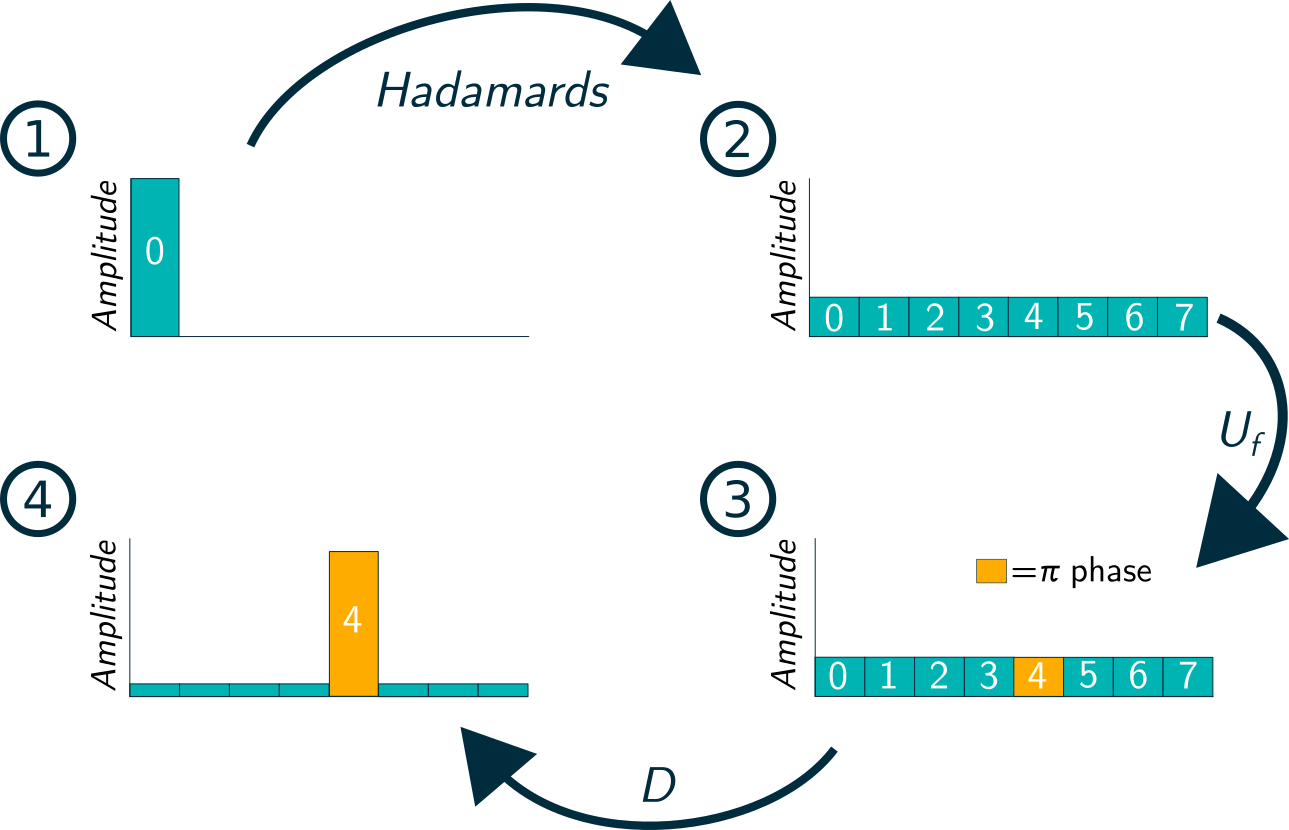
\includegraphics[width=0.9\linewidth]{figures/Grovers.png}
    \caption{Pictorial demonstration of the steps of Grover's Algorithm}
    \label{fig:Grovers}
\end{figure}


In the step 2 above, applying Hadamard gate to all the qubits leads to a state which is in superposition of all possible states (elements). It is important to start with the state $\ket{000}$ so that all the states in the superposition have the same initial phase. In step 3 we apply $U_{f}$ gate which is dependent on $f(x)$ and is able to recognise the marked element. What it does is that it applies a $\pi$ phase shift to the marked element but leaves all the other states unchanged. Next step is to apply gate $D$ to the state obtained in step 3. The application of gate $D$ can be understood as the operation which increases the amplitude of the phase shifted element in step 3. As mentioned in chapter 1, the measurement of a state leads to an output with a probability equal to the amplitude squared and thus, increasing the amplitude of the marked element state results in a higher probability of measuring that state. It is worth noting that repeating steps 3 and 4 a fixed number of times will increase the probability of detecting the marked element but after a certain point, the probability will start to decrease. For clarification, if we another iteration of step 3 and 4 in the above example, we get the state:
\begin{align}
\ket{\Psi}=\dfrac{-1}{8\sqrt{2}}\big(\ket{000}+\ket{001}+\ket{010}+\ket{011}-11\ket{100}+\ket{101}+\ket{110}+\ket{111}\big).
\end{align}
 Now if a measurement is performed on this state, there is a 94.53\% chance of getting the fifth element compared to 78.12\% probability if the measurement is performed after just one iteration. On the other side, if another iteration of step 3 and 4 is performed, the resulting state becomes:

\begin{align}
\ket{\Psi}=\dfrac{-7}{16\sqrt{2}}\big(\ket{000}+\ket{001}+\ket{010}+\ket{011}-\frac{13}{7}\ket{100}+\ket{101}+\ket{110}+\ket{111}\big)    
\end{align}
and the probability of getting the marked element upon measurement is only 67\% in this case. Therefore, it is important to choose the number of iterations for Grover's algorithm very carefully. The number of iterations ``$T$'' required to get the maximum probability of measuring the marked element is approximated as $T=\big(\pi\big/4)\sqrt{N}$.

%%%%%%%%%%%%%%%%%%%%%%%%%%%%%%%%%%%%
\subsubsection{General n-qubit case}

Given a function $f: \left\{0,1\right\}^n \rightarrow \left\{0,1\right\}$ with the promise that $f(x_0) = 1$ for a unique element $x_0$, the problem is to find this $x_0$. We use a quantum circuit on $n$ qubits with initial state $\ket{0}^{\otimes n}$.  Let $H$ denote the Hadamard gate, and let $U_0$ denote the $n$-qubit operation which inverts the phase of $\ket{0^n}$: $U_0\ket{0^n} = -\ket{0^n}$, $U_0\ket{x} = \ket{x}$ for all $x \neq 0^n$. The first step of the algorithm is to apply Hadamard gate on all $n$ qubits. Next, repeat the following operations T times for some T to be determined later.
%\begin{enumerate}
%\item Apply $H^{\otimes n}$.

%\item Repeat the following operations T times, for some T to be determined later:
\begin{enumerate}
\item Apply $U_f$, where $U_f\ket{x} = (-1)^{f(x)}\ket{x}$.
\item Apply $D$, where $D = -H^{\otimes n}U_0H^{\otimes n}$
\end{enumerate} 
%\item Measure all the qubits and output the result.
%\end{enumerate}
%\end{tcolorbox}
Finally, measure all the qubits and output the result.\\

In circuit diagram form, Grover's algorithm appears like: \\
\begin{equation*}
\Qcircuit @C=2.14em @R=1.25em
{\lstick{\ket{0}} & \gate{H} & \multigate{5}{U_f} & \multigate{5}{D} & \multigate{5}{U_f} & \ghost{U_f} & \lstick{\dots} & \multigate{5}{D} & \meter \\
\lstick{\ket{0}} & \gate{H} & \ghost{U_f} & \ghost{D} & \ghost{U_f} & \ghost{U_f} &\lstick{\dots} & \ghost{D} & \meter \\ 
& \dot{} & & & & & & & \dot{} \\
& \dot{} & & & & & & & \dot{} \\
& \dot{} & & & & & & & \dot{} \\
\lstick{\ket{0}} & \gate{H} & \ghost{U_f} & \ghost{D} & \ghost{U_f} & \ghost{U_f} & \lstick{\dots} & \ghost{D} & \meter \\}
\end{equation*}

\subsubsection{Construction of gate $D$ and $U_{f}$}
The gate $D$ in the algorithm applied on $n$-qubits can be implemented in the following manner. This shows that gate $D$ requires $2n+1$ Hadamard ($H$) gates, $2n+1$ Pauli $X$ gates and an n-control Toffoli gate.

\begin{align*}
\Qcircuit @C=1.14em @R=1.25em
{\lstick{\ket{x_1}} & \gate{H} & \gate{X} &  \ctrl{1} & \gate{X} & \gate{H} & \qw  \\
\lstick{\ket{x_2}} & \gate{H} & \gate{X} &  \ctrl{4} & \gate{X} & \gate{H} & \qw  \\
\lstick{\dot{}} & \dot{} & \dot{} & & \dot{} & \dot{} & \\
\lstick{\dot{}} & \dot{} & \dot{} & & \dot{} & \dot{} & \\
\lstick{\dot{}} & \dot{} & \dot{} & & \dot{} & \dot{} & \\
\lstick{\ket{x_n}} & \gate{H} & \gate{X} &  \ctrl{1} & \gate{X} & \gate{H} & \qw  \\
\lstick{\ket{0}} & \gate{x} & \gate{H} &  \targ & \qw & \qw & \qw }
\end{align*}

\vspace{1cm}
The construction of gate $U_{f}$ depends upon the function $f(x)$ being addressed by the algorithm.

%%%%%%%%%%%%%%%%%%%%%%%%%%%%
%%%%%%%%%%%%%%%%%%%%%%%%%%%%
%%%%%%%%%%%%%%%%%%%%%%%%%%%%
%%%%%%%%%%%%%%%%%%%%%%%%%%%%
\section{Quantum fourier transform}

Quantum Fourier transform (QFT) is the quantum analogue of discrete Fourier transform. It thus converts periodic functions to their conjugate domain (for example, time $\rightarrow$ frequency, position $\rightarrow$ momentum etc). Crucially it acts on quantum states. For example the QFT acting on two qubits is given by the transformation matrix 

\begin{align}
    QFT = 
    \frac{1}{2}
    \begin{pmatrix}
        \omega_N^{0} & \omega_N^{0} & \omega_N^0 &\omega_N^0 \\
        \omega_N^0 & \omega_N^1 & \omega_N^2 & \omega_N^3 \\
        \omega_N^0 & \omega_N^2 & \omega_N^4 & \omega_N^6 \\
        \omega_N^0 & \omega_N^3 & \omega_N^6 & \omega_N^9 \\
    \end{pmatrix}
    =
    \frac{1}{2}
    \begin{pmatrix}
        1 & 1 & 1 & 1 \\
        1 & i & -1 & -i \\
        1 & -1 & 1 & -1 \\
        1 & i & -1 & i \\
    \end{pmatrix}
\end{align}

This can be generalised to $n$ qubits, which requires a $2^n$ dimensional matrix with its elements given by 

\begin{align}
    QFT_{jk} = \omega_N^{jk} = \exp^{2\pi ijk / N} 
\end{align}

where we count the first columns and rows of the matrix from 0. The Quantum Fourier Transform can be constructed out of more fundamental quantum gates, a Hadamard gate and a controlled phase gate. 

 \begin{align}
    H = 
    \begin{pmatrix}
    1 & 1 \\
    1 & -1 \\
    \end{pmatrix},
    \quad
    R_n = 
    \begin{pmatrix}
    1 & 0\\
    0 & \omega_{2^n}\\
    \end{pmatrix}
 \end{align}
 
 This requires $n(n-1)/2$ controlled phase gates in total and $n$ Hadamard gates. 

The QFT is not an algorithm \textit{per se} but is crucial in many algorithms, such as Shor's algorithm as described in \ref{Shor's algorithm}.


%%%%%%%%%%%%%%%%%%%%%%%%%%%%%%%%%%

%%%%%%%%%%%%%%%%%%%%%%%%%%%%%
%%%%%%%%%%%%%%%%%%%%%%%%%%%%%
\section{Shor's algorithm}
%%%%%%%%%%%%%%%%%%%%%%%%%%%%%
%%%%%%%%%%%%%%%%%%%%%%%%%%%%%

\label{Shor's algorithm}

Shor's algorithm is a procedure to factor a large number. However, most of the steps in Shor's algorithm are in fact classical, and phrase the problem to be solved as one of finding the periodicity of a function. It uses a result from Euler that states that the The algorithm is given in box 

\begin{tcolorbox}[standard jigsaw,
    opacityback=0,  % this works only in combination with the key "standard jigsaw"
    boxrule=0.5pt,label={Shor's algorithm box}]
    {\bf Shor's algorithm}
    \tcbline
    \begin{enumerate}
    \item Pick a number $a<N$
    \item Calculate the greatest common divisor of this number $a$ and $N$, gcd($a,N$). If we obtain a number other than 1, then we have found a factor of $N$, so output gcd$(a,n)$ as our factor for $N$.
    \item Otherwise, find the period of the function $f(x) = a^x \mod N$. Label this period $r$
    \item Since  $a^0 \mod N = a^r \mod N = 1$, then $a^r - 1 \mod N = 0$. Factoring, $a^r-1 \mod N = (a^{r/2} - 1)(a^{r/2} + 1) \mod N = 0$. Thus $(a^{r/2} - 1)(a^{r/2} + 1) = lN$ for some integer $l$. If we found $r$ to be odd then this method has failed: return to 1. 
    \item Output either gcd($a^{r/2}-1$) or gcd($a^{r/2}+1$) as the factors of $N$.
    \end{enumerate}
\end{tcolorbox}

However, step 3 is not efficient classically. We can however use a quantum algorithm to provide a polynomial speed-up. We shall now explain to explain the machinery behind this process, attempting to develop an intuition for the quantum effects over the fine detail of this process. The diagram demonstrates the processes which occur. 


[DIAGRAM OF AMPLITUDES AND PHASES GO HERE, FOLLOWED BY EXPLANATION]



The circuit shown below implements Shor's algorithm. The $1^{st}$ register uses Hadamard gates to put the qubits in a uniform superposiiton. The second step uses an Oracle operation $U_f$ for a periodic function $f=a^x \mod N$ which has the following effect on the first and second registers:

\begin{align}
    U_f\ket{x}\ket{0} = \ket{x}\ket{f(x)}
    U_{a^x\mod N}\ket{x}\ket{0} = \ket{x}\ket{a^x\mod N}
\end{align}


measuring the second register then collapses it to a single $f_0 = f(x_0)$, where $f(x_0) = f(x_0 + r) = f(x_0 + 2r) = ...$ for the periodicity $r$ of the function. Thus the first register, through entanglement, is now in the a superposition of the states $\ket{x_0+jr}$ for all integers $j$ allowed for $x_0+jr$ to be within the register. Therefore we have a periodic superposition of a state, generating peaks in the spectrum as can be seen in [REF TO DIAGRAM TO BE ADDED]. This is a problem that can be clearly solved by the QFT - we have states that are periodic with period $r$ in one (Hilbert) space, and applying the inverse QFT will obtain a single strong peak at $r$.

\begin{figure}
\begin{align*}
\Qcircuit @C=2.14em @R=1.8em
{
& & & \lstick{\ket{0}} & \gate{H} & \multigate{7}{U_f} & \qw & \multigate{4}{QFT^{-1}} & \meter \\
& & &\lstick{\vdots} & \vdots &                         &              &         & \lstick{\vdots}  \\
& \push{\mathrm{1^{st}\,register}} & &\lstick{\ket{0}} & \gate{H} &           \ghost{U_f} & \qw &\ghost{QFT^{-1}} & \meter \\
&   &&\lstick{\ket{0}} & \gate{H} &           \ghost{U_f} & \qw &\ghost{QFT^{-1}} & \meter \\
&                   &&\lstick{\ket{0}} & \gate{H} &           \ghost{U_f} & \qw &\ghost{QFT^{-1}} & \meter \\
&                   &&\lstick{\ket{0}} & \qw &               \ghost{U_f} &  \meter \\
& \push{\mathrm{2^{nd}\,register}}              & &\lstick{\vdots} &       &                   &\lstick{\vdots} \\
&                   &&\lstick{\ket{0}} & \qw &       \ghost{U_f} & \meter  \gategroup{1}{3}{5}{3}{1.7em}{\{}
\gategroup{6}{3}{8}{3}{1.7em}{\{}}
\end{align*}
\caption{This circuit implements Shor's algorithm.}
\label{fig:apprPerAlgAlternative}
\end{figure}


\begin{sidewaystable}
\begin{tabular}{|c|c | c | c |c|}
    \hline
    \thead{Algorithm \\ name} & \thead{Purpose} & \thead{Number of \\qubits used} & \thead{Number of \\gates required} & \thead{Probability\\ of success}  \\
    
    \hline
    
    \makecell{Grover's \\algorithm} & \makecell{Unstructured \\search} & \makecell{$n$ qubits for \\$2^n$ marked \\elements} & \makecell{$(2T+1)n$ Hadamard gates,\\$T$ $U_f$ gates, and $T$ $U_0$ gates, \\where $T \approx \frac{\pi}{4} \sqrt{2^n}$} & $\sin^2((2T+1)\arcsin{\frac{1}{\sqrt{2^n}}})$\\
    \hline
    
    \makecell{Quantum period \\finding\\} & \makecell{Finding \\Periodicity} &  & & \\
    \hline
    
    \makecell{Deutsch-Jozsa\\algorithm\\} & \makecell{Constant or \\Balanced function} & \makecell{$n+1$ qubits for\\$2^n$ elements} & \makecell{One $U_{f}$ gate and\\$2n+1$ Hadamard gates}& \makecell{100\%}\\
    \hline
    
    \makecell{Eigensolver} & & & & \\
    \hline
    
    \end{tabular}
\end{sidewaystable}